\documentclass[runningheads]{llncs}
%
\usepackage{paralist}
\usepackage{comment}
\usepackage{hyperref}
\usepackage{graphicx}
\usepackage{algorithm}
\usepackage{algpseudocode}
\usepackage{color}
\definecolor{blue}{RGB}{42,0,255}
\definecolor{green}{RGB}{63,127,95}
\definecolor{purple}{RGB}{127,0,85}
\definecolor{lime}{RGB}{114, 148, 0}
\usepackage{listings}
\lstdefinelanguage{Cryptol}{
  keywordstyle=[1]\color{blue}\bfseries,
  keywordstyle=[2]\color{purple}\bfseries,
  keywordstyle=[3]\color{black}\bfseries,
  basicstyle={\color{lime}\scriptsize},
  literate=*
  {*}{{{\color{black}$*$}}}{1}
  {=}{{{\color{black}=}}}{1}
  {+}{{{\color{black}+}}}{1}
  {-}{{{\color{black}$-$}}}{1}
  {\%}{{{\color{black}\%}}}{1}
  {(}{{{\color{black}(}}}{1}
  {)}{{{\color{black})}}}{1}
  {\{}{{{\color{black}\{}}}{1}
  {\}}{{{\color{black}\}}}}{1}
  {[}{{{\color{black}[}}}{1}
  {]}{{{\color{black}]}}}{1}
  {|}{{{\color{black}$|$}}}{1}
  {>}{{{\color{black}$>$}}}{1}
  {<}{{{\color{black}$<$}}}{1}
  {\#}{{{\color{black}\#}}}{1}
  {@}{{{\color{black}@}}}{1}
  {.}{{{\color{black}.}}}{1}
  {\'}{{{\color{black}'}}}{1}
  {:}{{{\color{black}:}}}{1}
  {^}{{{\color{black}$\char`\^$}}}{1}
  {&}{{{\color{black}\textbackslash}}}{1},
  morekeywords=[1]{Bit, Integer, STATE_ARR, W, COL, type, LIST4, LIST63, True, False},
  morekeywords=[2]{if, then, else, where},
  morekeywords=[3]{pi, rc, cond, a, b, x, y, z, for, n, r, R, f, rs, i, index, t, 
    vals, loop, state, while, take}
}

\definecolor{dkgreen}{rgb}{0,0.6,0}
\definecolor{almond}{rgb}{0.94, 0.87, 0.8}
\definecolor{amaranth}{rgb}{0.9, 0.17, 0.31}
\definecolor{azure}{rgb}{0.0, 0.5, 1.0}
\definecolor{gray}{rgb}{0.5,0.5,0.5}

\lstdefinestyle{customc}{
  frame=none,
  language=C,
  basicstyle=\footnotesize\ttfamily, 
  aboveskip=3mm,
  belowskip=3mm,
  showstringspaces=false,
  numbers=left,
  keywordstyle=\bfseries\color{azure},
  commentstyle=\itshape\color{dkgreen},
  identifierstyle=\color{black},
  stringstyle=\color{almond},
  numbersep=-1pt,
  numberstyle=\color{gray},
  breaklines=true,
  breakatwhitespace=true,
  tabsize=3,
}

% Used for displaying a sample figure. If possible, figure files should
% be included in EPS format.
%
% If you use the hyperref package, please uncomment the following line
% to display URLs in blue roman font according to Springer's eBook style:
\renewcommand\UrlFont{\color{blue}\rmfamily}
\newcommand\keccak{\textsc{Keccak}}
\newcommand\shaThree{\texttt{SHA-3}}
\newcommand\nist{\texttt{NIST}}
\newcommand\fips{\texttt{FIPS 202}}
\newcommand\saw{\texttt{SAW}}
\newcommand\cryptol{Cryptol}
\newcommand\openssl{OpenSSL}
\newcommand{\figref}[1]{Fig.~\ref{#1}}
\newcommand{\algoref}[1]{Alg.~\ref{#1}}
\newcommand{\lineref}[1]{Line~\ref{#1}}

\begin{document}
%
\title{Verification of OpenSSL's SHA3 \keccak\ function using the Software Analysis Workbench}
%
%\titlerunning{Abbreviated paper title}
% If the paper title is too long for the running head, you can set
% an abbreviated paper title here
%
\author{
  Parker Hanson\inst{1} \and
  Benjamin Winters\inst{1} \and
  Eric Mercer\inst{1}\orcidID{0000-0002-2264-2958} \and
  Bret Decker\inst{1}
}
%
\authorrunning{P. Hanson et al.}
% First names are abbreviated in the running head.
% If there are more than two authors, 'et al.' is used.
%
\institute{
  Brigham Young University, Provo UT 84602, USA
}
%
\maketitle              % typeset the header of the contribution
%
\begin{abstract}
\shaThree\ is the new standard from \nist\ for computing digests. 
\openssl\ is one of the most widely used implementations of cryptographic protocols.
\cryptol\ and the Software Analysis Workbench (\saw) are a language and verification engine to specify cryptographic primitives and prove equivalence to implementations.
As digests are the basis for all cryptographic protocols, the research in this paper is an automated \saw\ proof of equivalence between the \shaThree\ standard and the actual \openssl\ implementation in C.
The research contributes \cryptol\ specifications for the published standard and the \openssl\ implementation of the standard with its several changes.
The equivalence proof shows the importance of overrides in \saw\ to replace C code with \cryptol\ to reduce the complexity of the proof obligations that must be accomplished relative to the implementation in C.
The research establishes the viability of verifying modern cryptographic primitives and the importance of modularity in their definitions, and implementations, for overrides.

% The \keccak\ function in the SHA-3 NIST standard is responsible for the major computations of all SHA-3 hash constructs.
% These constructs form the basis for modern secure hashing.
% This work extends and improves the methodology used to verify Amazon's s2n HMAC and OpenSSL's SHA2-256 inner hash function. 
% It uses the Software Analysis Workbench (SAW) to prove out functional equivalence between OpenSSL's SHA-3 Keccak function and a verified implementation of SHA-3 in Cryptol, a domain-specific language for cryptography. 
% SAW allows for a modular approach to writing proofs through the use of contracts, which define a functions input to output relationship.
% Each contract, also called an override, is an obligation in the full proof.
% This work leverages SAW by creating overrides to decompose computation and create a compositional proof that is within the capacity of an SMT solver. 
% Visual inspection between Cryptol and the NIST standard is simplified through the creation of Cryptol utility functions.
% These utility functions wrap the complex list comprehensions required for looping in Cryptol.
% The results of this work indicates that a modular approach in cryptographic algorithm design greatly simplifies the verification process, as exemplified by SHA-3.

\keywords{verification \and cryptography \and symbolic execution \and SHA3.}
\end{abstract}

\section{Introduction}\label{sec:introduction}
This paper discusses an automated proof of the \emph{Secure Hash Algorithm 3} (\shaThree) in \openssl\ using the \emph{Software Analysis Workbench} (\saw) by Galois.
\shaThree\ is the latest algorithm for computing \emph{digests}, or hashes, from data to be published by the \emph{National Institute of Standards and Technology} (\nist).
The algorithm is the successor to \shaTwo.
Its intent is to address weaknesses in \shaTwo, and it departs from its predecessors in that it is based on the \keccak\ family of cryptographic primitives \cite{fips202}.

\openssl\ is a commercial grade free cryptographic library \cite{openssl}.
Its implementation of the \emph{Secure Sockets Layer} (SSL) and \emph{Transport Layer Security} protocols are widely deployed on internet facing applications.
Computing digests is a critical operation in these protocols and is the basis to the security guarantees provided by these protocols.
Widely deployed implementations, such as \openssl, are especially important to be correct because of the available attack surface to hackers if a vulnerability were discovered in such implementations.
The seriousness of getting these implementations correct is recently seen in the Apache \texttt{log4j} vulnerability affecting virtually all internet facing servers \cite{log4j}.

\saw\ is a formal verification tool to prove equivalence between \sawcore\ models. \sawcore\ models are defined in the \cryptol\ functional language or extracted from C or Java with \emph{symbolic execution}.
\cryptol\ itself is designed to specify cryptographic primitives at the bit level.
\saw\ has been shown capable in proving implementations of cryptographic primitives equivalent to hardware and software implementations \cite{crypt-hi,hard-soft,design-verif}.
Recent work emphasizes not just the utility of \saw, but the importance of modular decomposition of cryptographic primitives in their definition as that decomposition lends itself to efficient verification in \saw\ \cite{nfm-us}. 

This paper details another example of \saw\ verification only this time it is a proof showing the \openssl\ C implementation of \shaThree\ matches a \cryptol\ specification derived from the published \fips\ standard by \nist\ \cite{fips202}.
The \cryptol\ specifications, \saw\ scripts, and extracted \sawcore\ model from the \openssl\ C implementation are documented, and available, in a public GitHub repository for independent verification \cite{sha3proof}.
The proof relies on two specifications, both created as part of this research, of the \shaThree\ algorithm: one that closely matches the published standard and another incorporating features in the C implementation.
\saw\ shows an input to output equivalence between these two specifications for the 256 bit digest over a fixed set of message sizes. The proof takes around 60 hours of computation time.

The proof then turns to the inner \keccak\ function that computes the actual bits for the digest.
Here it shows that the C implementation exactly matches the \cryptol\ specification on any input.
The proof requires the use of \emph{overrides} in \saw\ to simplify the extracted model from C after symbolic execution.
The proof of equivalence between the \keccak\ in C and \cryptol\ takes around 15 minutes of computation time.

The proof, with its artifacts in the published repository, make the following contributions:
\begin{compactitem}
  \item \cryptol\ for \shaThree\ that passes the test vectors and correlates with \fips.
  \item \cryptol\ for \shaThree\ that uses a reordered memory layout and precomputed tables that correlate with C implementations.
  \item A \saw\ proof showing the two specifications equivalent for the 256 bit digest over a series of message sizes.
  \item A \saw\ proof that the \keccak\ specification in \cryptol\ is equivalent to the \openssl\ C implementation of the same function for all inputs.
\end{compactitem}
The proof shows that \saw\ is capable of proving equivalence to C implementations of modern cryptographic primitives.
It also shows that the modular definition of \shaThree\ naturally lends itself to formal verification in \saw.
The work in its entirety argues the importance of using formal languages such as \cryptol\ for the specification of cryptographic primitives rather than English prose and math.
It also argues the necessity, and viability, of proving at the intermediate representation level equivalence between cryptographic specifications and actual C implementations.

\begin{comment}
\noindent \textbf{Limitations}
\begin{compactitem}
  \item Visual inspection and limited test vectors for (1) and (2)
  \item Only provide proof certificates for message sizes of X to Y for digest sizes of \textbf{FIXME} for (3)
  \item Visual inspection only for anything above Keccak for (3) in OpenSSL's C-code
\end{compactitem}

\subsection{Related Work}
  Previously, Galois' Inc. worked with Amazon to prove out parts of Amazon's s2n HMAC code to the NIST specification.  
In their work they stubbed out use of the SHA2 algorithm because their HMAC allows for customization of the algorithm type and implementation.

The work by Decker et. al, extended on Galois' work by choosing a single SHA2 implementation to prove out.  
They chose OpenSSL's SHA 256 implementation, as that is a commonly used library (and one that is usable in s2n).  
They were able to prove out the inner hash computations of that implementation using a methodology of compositional proofs to do so.  
They were also able to connect up their proof with the code used by Galois' to stub out the SHA2 algorithm, which implies that the functional equivalence property established with the OpenSSL code applies to Galois' Cryptol implementation as well.  
Their work showed the viability and limitations of creating proofs of functional equivalence for legacy cryptographic implementations.



\subsection{SHA 3}
This work shows that this same methodology can be extended to modern cryptographic algorithms.
The SHA 3 family of algorithms is defined by NIST in the FIPS 202 publication.
It specifies a block hashing algorithm, Keccak, that is used by each of the different SHA and SHAKE algorithms.
In comparison to the SHA 2 family of algorithms, Keccak features significantly more complex and robust computations.
This increase in computation was of interest, because it presses the limits of SAW's capabilities.

\subsection{Results}
This work shows a complete proof of functional equivalence from a verified implementation of the NIST standard to OpenSSL's C code for the Keccak function.
In doing so, it shows SAW's ability to stand up against more difficult computations.
It also provides insights into using Cryptol's functional nature to further simplify the step of visually verifying Cryptol code to the NIST standard.

Because of how NIST defines the standard, the keccak function is used for each digest size of the SHA3 algorithm, with the only significant differences being in the padding/sponging parts of the algorithm, which falls outside this work's scope.
This means that the proof of correctness for this function extends usefulness beyond just the SHA3-256 level which we focused on.
In our repository, we wrote the Cryptol specification to be able to run any of the SHA3 family of algorithms using the same keccak.
A simple extension of this work would be to take that already created and verified Cryptol specification, and prove it up against OpenSSL's slightly modified keccak versions.
\end{comment}

\section{Background}\label{sec:background}
\cryptol\ and \saw\ are used to prove properties of \openssl's implementation of \shaThree\ relative to the \nist\ \fips\ publication \cite{fips202}. 
What the proofs actually say, and an understanding of their limitations, relies on (1) a basic knowledge of how \saw\ works and what \cryptol\ does relative to \saw, and (2) how the \shaThree\ algorithm constructs its digests.
Key elements relative to understanding the proof of each (\cryptol, \saw, and \shaThree) are defined in this section. 

\subsection{Cryptol and SAW}\label{subsec:saw}
\cryptol\ is a domain specific functional language for describing cryptographic primitives, such as algorithms to compute digests, at the bit-level.
Cryptographic primitives are the building blocks for complex cryptographic protocols, such as SSL, that provide a broad range of security guarantees.
\cryptol\ is executable, being able to run test vectors to validate specifications, and more importantly, it compiles directly to \sawcore\ which is the language for formal models in \saw.

\saw\ is a tool to extract formal models from programs with support for C, Java, and \cryptol\ input.
These formal models are expressed in the \sawcore\ language that supports formal reasoning.
As mentioned previously, \cryptol\ compiles directly to \sawcore, but that is not the case for C and Java.
\saw\ uses \emph{symbolic execution} to extract \sawcore\ models from C and Java inputs.

Symbolic execution reasons about all computation paths in the C or Java input.
It must unroll all loops a static number of times to create the model in \sawcore.
As such the number of iterations in any loop must be statically known at compile time or the symbolic execution fails to terminate.
\sawcore\ models from symbolic execution tend to be more complex than those from \cryptol.

\saw's function, among other things, is to prove input to output equivalence between \sawcore\ models.
It accomplishes such proofs with equivalence preserving rewrites on the \sawcore\ and with automated reasoning.
The rewrites simplify the \sawcore\ models as size correlates with complexity in the automated reasoning. 
The rewrites also try to structurally reduce one model to the other thus avoiding automated reasoning altogether.
When rewriting is not sufficient, the equivalence between two models is reduced to a satisfiability problem and dispatched to external backend solvers.

\saw\ supports hierarchical reasoning with \emph{overrides}.
An override replaces one \sawcore\ model with another in the formal analysis.
As an example, consider a Java method that itself calls another Java method as part of its implementation.
Suppose that \saw\ is able to prove that a \cryptol\ specification for the called method and the Java implementation of the same method are equivalent.
If that is possible, then an override is able to replace the called Java method with the \sawcore\ from the \cryptol\ and as a result avoid any symbolic execution of that method when creating the \sawcore\ model of the Java.

As mentioned previously, \sawcore\ from \cryptol\ is less complex than equivalent models created by symbolic execution from C or Java; thereby overrides reduce the overall complexity of the final extracted \sawcore\ models from C or Java.
As such, proving a property about a complex C function or Java method generally requires the use of overrides from \cryptol\ in order for the equivalence proof to be successful, and that is regardless of how that proof is accomplished.
Overrides improve the likelihood of the rewrites showing equivalence and the likelihood of the backend solver being able to show equivalence if the rewrites fail.
Indeed, the use of overrides are key to the \saw\ proof in this paper showing equivalence between the \shaThree\ specification and the \openssl\ C implementation.

\subsection{SHA-3 Overview}\label{subsec:sha3}
\begin{algorithm}[t]
  \caption{\shaThree\ sponge construction with \keccak}\label{alg:sha3}
  \begin{algorithmic}[1]
    \Require $n \geq 0$ and $(d,r) \in \{(224, 1152)\ (256, 1088)\ (384, 832)\ (512, 576)\}$
    \Ensure $D =$ \shaThree(N,d,r)
    \State $p_0, \ldots, p_m = \mathtt{pad}(N, r)$\label{line:pad}
    \State $S = 0_0, \ldots, 0_{1599}$\label{line:init}
    \For{$p_i = p_0, \dots, p_m$}
      \State $S = S\ \mathbf{xor}\ \mathtt{zeroExtend}(p_i, s-r)$\label{line:absorb}
      \State $S =$ \keccak$(S)$\label{line:keccak}
    \EndFor
    \State $D = \mathtt{squeeze(S,d)}$\label{line:squeeze}
  \end{algorithmic}
\end{algorithm}

\shaThree\ uses \emph{sponge construction} to generate hashes as shown in \algoref{alg:sha3} (see \nist\ \fips\ \cite{fips202}).
Sponge construction \emph{absorbs} data into an internal state $S$ at a rate of $r$ bits per cycle (\lineref{line:absorb} and \lineref{line:keccak}), transforming the state on each cycle, and once all the data is absorbed, then it \emph{squeezes} out a final $d$-bit digest (\lineref{line:squeeze}).
The transformation function, \keccak-f[1600], simply \keccak\ in the rest of this presentation, defines the size of the state $S$ to be $s = 1600$ bits, which is initialized to 0 (\lineref{line:init}).

The state itself consists of $r$ bits that are written or read plus a capacity of $c = s - r$ bits that are untouched by input or output.
The \nist\ standard defines pairs of allowed hash sizes and rates.
These are defined in the requires statement in \algoref{alg:sha3}. 
The input $N$ is padded such that its final size is a multiple of $r$ bits, and it is partitioned into $r$-bit size blocks (\lineref{line:pad}) for the absorption phase.
The padding is defined by the regular expression $10^*1$.
Padding is always added to $N$ even if adding it creates an extra block.

The \keccak\ transformation function takes place over twenty-four rounds with each round consisting of five steps: $\theta$, $\rho$, $\pi$, $\chi$, and $\iota$.
The state $S$ itself is viewed as a $5 \times 5$ array of $64$-bit words (e.g. $5 * 5 * 64 = 1600$) in each of the steps.
$\theta$ computes a parity over the columns in the state. $\rho$ is a bitwise rotate over the state.
$\pi$ is a permutation on the state. $\chi$ is a non-linear operation that combines along the rows in the state.
And $\iota$ mixes in twenty-four different constants, one for each iteration, into portions of the state.



\section{Proof Outline and Results}\label{sec:proof}
SHA 3 Details
\begin{figure*}[ht]
  \centering
  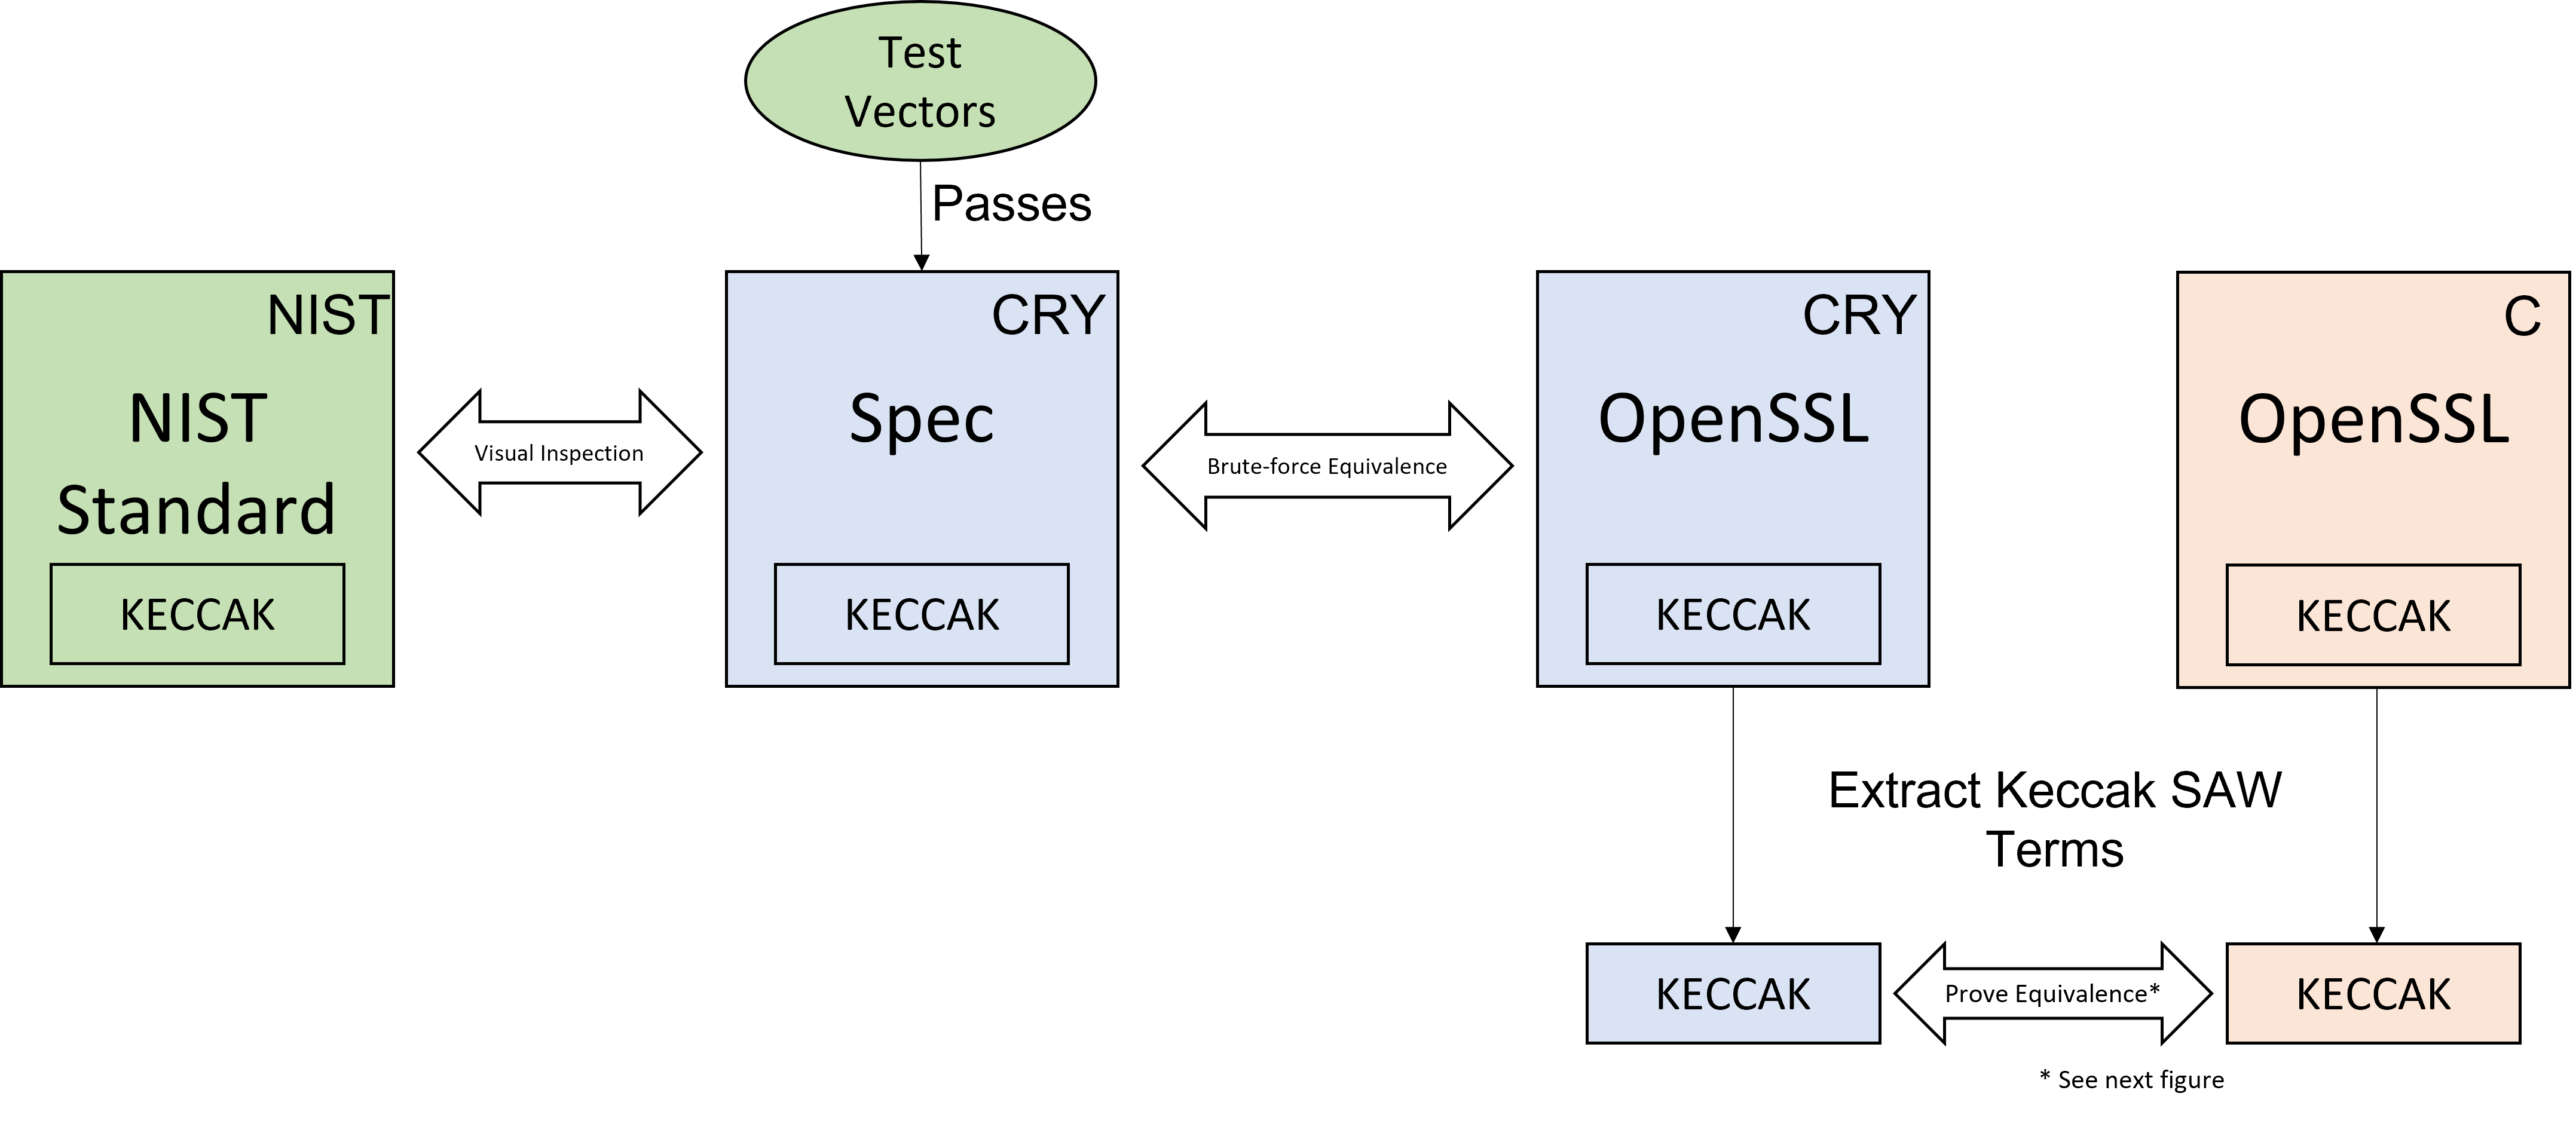
\includegraphics[width=\linewidth]{figs/proof.png}
  
  \caption{SHA3 Keccak Proof Structure}
  \label{fig:proofStructure}
  
\end{figure*}
\begin{figure*}[ht]
  \centering
  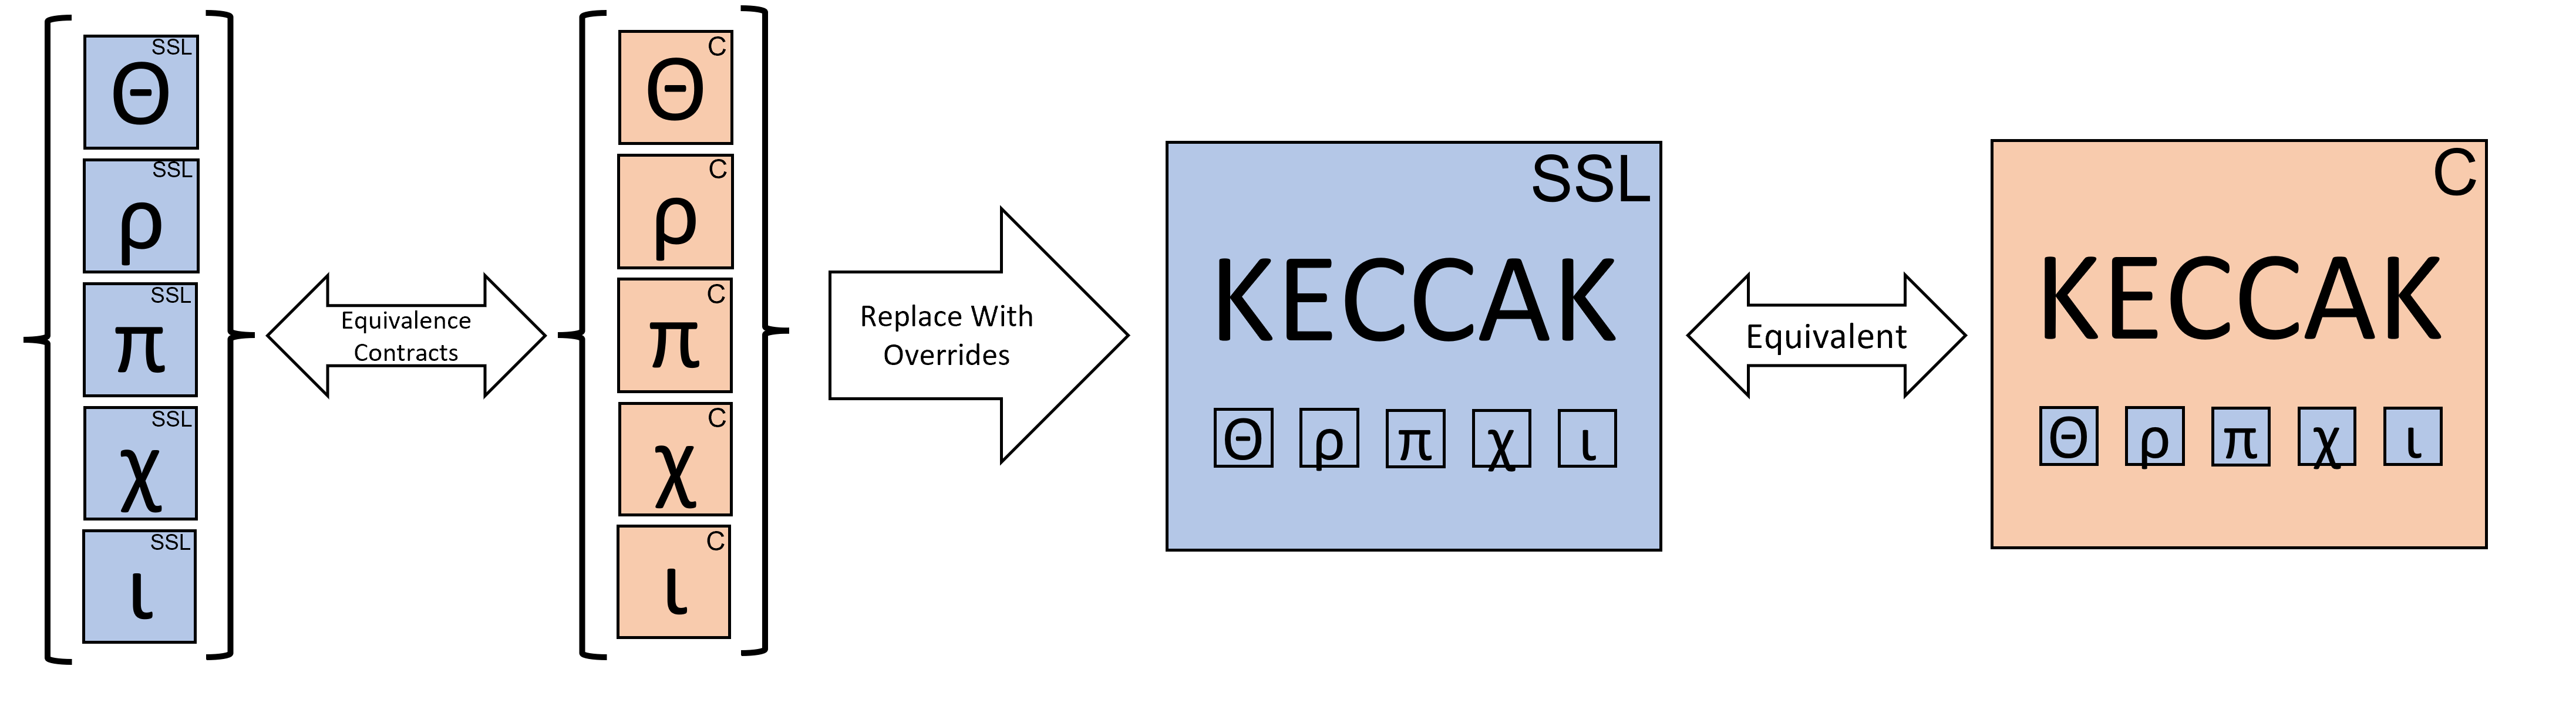
\includegraphics[width=\linewidth]{figs/proof2.png}
  
  \caption{Inner Function Contracts}
  \label{fig:proofStructure2}
  
\end{figure*}

\begin{compactitem}
  \item Process 1600 bits at a time: $5 * 5 * 64$
  \item State vector is $5*5*64*$
  \item Incoming message padded out to whole number of 1600 bit bit-strings
  \item Processed in order by \texttt{KECCAK}
  \item Keccak turns each block into a state vector (rearranges bit layout in memory)
  \item Keccak has 24 rounds for state vector. 
  \item There are 5 hash functions sequentially applied in each round to iteratively update the state vector
  \item After the last round, keccak turns the state vector back into the bit-string./\item The next unprocessed block is \emph{sponged} (e.g., absorbed) into the current bit-string from the latest keccak and the process is repeated 
  \item The max digest (hash) size is 512 bits in the standard
  \item The final bit-string from keccak after sponging and processing every block in the original message is truncated to the desired digest size 
\end{compactitem}

SAW Details
\begin{compactitem}
  \item Cryptol is a specification language specifically for defining crypto-primitives
  \item It has a compiler to turn Cryptol to SAW core terms
  \item It has an execution environment to run test vectors on specifications
  \item SAW is a tool to prove equivalence between SAW core terms
  \item It uses symbolic execution and must unroll every loop to a fixed length
  \item It can take as input C and Java code and compile those to core terms
  \item It can use overides to replace C and Java code in the term
\end{compactitem}

SAW provides a verification environment for compositional proofs of functional equivalence between two pieces of supported code (C, Java, or Cryptol).
SAW uses symbolic execution to create computational models of the code and creates problems of functional equivalence between those two models that can be pushed off to an SMT solver.  
The difficulty of these SMT problems is directly affected by the size and complexity of the computations that are being compared.
This can lead to drastic increases in proof times and sometimes even prevents completion as computations increase.  
SAW's solution to this is to create contracts (called overrides) of a functions input to output relationship which allows for a modular approach to writing the proof.
By breaking up computation into smaller pieces, and creating overrides for these pieces, SAW can often simplify an otherwise complex (and thus incompletable) proof to remain within the capacity of an SMT solver.

Cryptol is a domain-specific specification language, which has been used in the previously mentioned works by Galois' and by Decker et. al to write visually reviewable implementations of NIST standards.
It has strong ties to the SAW tool and, in fact, can be compiled directly down to the SAW Terms (computational models) which are used by SAW in proving functional equivalence.
Because of the interwoven nature of Cryptol with SAW, the Terms created from Cryptol are in most cases significantly simpler than any created through symbolic execution of C/Java code.

The published NIST standards provide no compileable implementation that can be used as a starting point for proving out the algorithm.
As a result, any proof of correctness with a NIST standard is limited in strength to how simple it is use visual review to connect code used in the proof to the NIST standard, coupled with a small sampling of test vectors.
As shown in \ref{proofStructure}, The proof flow starts with a specification of the SHA3 algorithm in Cryptol with the goal of being as similar visually to the NIST standard as possible.
This work discusses significant ways that Cryptol's functional nature can be leveraged to aid in this goal.
Along with simplifying the visual inspection process, this Cryptol specification also passes all test vectors provided by NIST.

The end goal of this proof is to show functional equivalence between this visually reviewable specifications Keccak function, and that of OpenSSL's C code.
Unfortunately, a direct proof between this specification, and OpenSSL's implementation proved unfeasible, because OpenSSL varies from the NIST standard in how it stores the bits of the intermediate state array in memory.
These minor modifications in memory storage put such a proof out of SAW's capabilities, because it relies on strict typing, and comparison of a Cryptol functions input/output to a C functions memory state.
In order to bridge that gap, a second Cryptol specification is included in the proof flow.
It matches in every way the first Cryptol code, except when it comes to how the state array is stored and accessed (at which point it follows OpenSSL's form).
Because of the efficient nature of Cryptol's compilation to SAW Terms, proving equivalence between these Cryptol implementations was possible at the top level of the SHA3 algorithm (which allows for the differences in state array storage to be fully abstracted out).
Due to the strict typing nature required for writing SAW proofs, the scope of this equivalence proof is limited to a given input message size.
The only computations that change in the SHA3 algorithm due to message size are in the padding and sponging of a block.
With this in mind, an exhaustive proof run over each input message byte count from 1 to the block size is sufficient to cover the differences in computation.
The artifact repository accompanying this work contains the receipts of this exhaustive proof. (REFERENCE TO PROOF!!!!)

INNER GREEK FUNCTIONS:

CONTRACTS CAN BE USED TO OVERRIDE AND REPLACE C WITH Cryptol

WITH THESE CONTRACTS SAW CAN COMPLETE A PROOF OF EQUIVALENCE BETWEEN TWO PIECES OF CODE.

This work relies on the correctness of several tools, including language compilers. 

\noindent \textbf{Trusted Code Base}:
\begin{itemize}
  \item LLVM bitcode compiler
  \item The Software Analysis Workbench (SAW) including the conversion from LLVM bitcode to SAWCore terms, the Cryptol compiler to SAWCore terms, and SAW's interface with SMT solvers.
  \item The z3, abc, and yices SMT solvers.
\end{itemize}


\section{FIPS 202 Specification in Cryptol}\label{sec:fips}
This section illustrates with a few examples how the \fips\ specification is captured in \cryptol. 
\cryptol's list comprehensions do not directly align with the quantification and iteration in the specification. 
This misalignment makes the \cryptol\ specification more difficult to read and to manually argue its equivalence relative to the published specification.
The two specifications are better aligned through a library of two methods in \cryptol\ that hide the list comprehensions so that the \cryptol\ specification reads more like the \fips\ specification. The two library methods are the \emph{for-method} and the \emph{while-method} discussed in this section.

\subsection{The for-method}

\newsavebox{\fipsPi}
\begin{lrbox}{\fipsPi}
  \begin{lstlisting}[basewidth = {.5em},basicstyle={\small}]
    1. For all triples (x,y,z) such that 
           0 <= x < 5, 0 <= y < 5, and 0 <= z < w,
       let A'[x, y, z] = A[(x + 3y) mod 5, x, z].
    2. Return A'.
  \end{lstlisting}
\end{lrbox}

\newsavebox{\PiCry}
\begin{lrbox}{\PiCry}
  \begin{lstlisting}[language=Cryptol, numbers=left, escapeinside={;}{;}]
    type STATE_ARR = [5][5][64];\label{line:pistate};
    pi : STATE_ARR -> STATE_ARR
    pi a = [  [  [a @x @((x + 3*y) % 5) @z;\label{line:pi};
                 | z <- [0..63]];\label{line:list};
              | y <- [0..4]] 
           | x <- [0..4]]
  \end{lstlisting}
\end{lrbox}

\newsavebox{\PiCryLib}
\begin{lrbox}{\PiCryLib}
  \begin{lstlisting}[language=Cryptol]
    pi a = for [0..4] (&x ->
             for [0..4] (&y -> 
               for [0..63] (&z -> 
                 a @x @((x + 3*y) % 5) @z)))
  \end{lstlisting}
\end{lrbox}

\newsavebox{\formethod}
\begin{lrbox}{\formethod}
  \begin{lstlisting}[language=Cryptol]
    for : {n, a, b} [n]a -> (a -> b) -> [n]b
    for vals f = [f i | i <- vals]
  \end{lstlisting}
\end{lrbox}

\begin{figure}[t]
  \begin{center}
    \begin{tabular}{l}
      \usebox{\fipsPi} \\ \\
      \multicolumn{1}{c}{(a)} \\ \\
      \usebox{\PiCry} \\ \\
      \multicolumn{1}{c}{(b)} \\ \\
      \usebox{\formethod} \\ \\
      \multicolumn{1}{c}{(c)} \\ \\ 
      \usebox{\PiCryLib} \\ \\
      \multicolumn{1}{c}{(d)}
    \end{tabular}
  \end{center}
  \caption{The $\pi$ function. (a) The \fips\ specification. (b) The \cryptol\ with comprehensions. (c) The for-method definition. (d) The \cryptol\ with the for-method.}
  \label{fig:pi}
\end{figure}

A common idiom in the \fips\ publication is using quantification over a finite domain defined by linear constraints to define input for some computation.
The definition of the $\pi$ function for \keccak\ shown in \figref{fig:pi}(a) is one such example.
Here the quantification is used to define the set of indices that are part of the $\pi$ computation that transforms the state array. The intent is that of a \emph{parallel-for} where order does not matter since the new state array $A^\prime$ only depends on the old state array $A$.

The \cryptol\ definition using list comprehensions is given in \figref{fig:pi}(b).
\lineref{line:pistate} defines the state as a $5 \times 5$ array of 64-bit words.
\lineref{line:pi} starts the definition of $\pi$. 
Here the comprehensions are nested with the list indices appearing in reverse order to follow the nesting.
\lineref{line:list} gives the domain for $z$ as a list with values from 0 to 63.
The domains for $x$ and $y$ are given similarly.
The domains for $x$, $y$, and $z$ all match the domains defined in the quantification in \figref{fig:pi}(a).
Although the list comprehensions are not unreadable, the \cryptol\ can be improved by creating a for-method to hide some of the details.

\figref{fig:pi}(c) is the \cryptol\ definition of the for-method.
It takes two arguments: a list, \emph{vals}, for the comprehension, and a function, $f$, to apply to each element of the list.
Its definition is as expected: it creates a new list that is the result of applying $f$ to each element in \emph{vals}.

\figref{fig:pi}(d) is the rewritten \cryptol\ using the for-method.
It still requires the indices lists for the list comprehensions, but it has a more obvious correspondence to the original definition in \figref{fig:pi}(a).
The for-method reorders and structures the arguments in a very elegant way.
It hides the list comprehensions to simplify the task of visual inspection for equivalence.

\subsection{The while-method}

\newsavebox{\fipsRc}
\begin{lrbox}{\fipsRc}
  \begin{lstlisting}[basewidth = {.5em},basicstyle={\small}]
    1. If t mod 255 = 0, return 1.
    2. Let R = 10000000.
    3. For i from 1 to t mod 255, let:
      a. R = 0 || R;
      b. R[0] = R[0] ^ R[8];
      c. R[4] = R[4] ^ R[8];
      d. R[5] = R[5] ^ R[8];
      e. R[6] = R[6] ^ R[8];
      f. R = Trunc8[R].
    4. Return R[0].
  \end{lstlisting}
\end{lrbox}

\newsavebox{\RcCry}
\begin{lrbox}{\RcCry}
  \begin{lstlisting}[language=Cryptol, numbers=left, escapeinside={;}{;}]
    rc : [64] -> Bit
    rc t =  if (t % 255) == 0 then 1
            else rs !0 @0 where;\label{line:return};
              rs = [0b10000000] #;\label{line:init};
                   [if i <= t % 255 then;\label{line:compute};
                      (take'{8} ([(r@0) ^ (r@8),
                                   r@1, r@2, r@3, 
                                  (r@4) ^ (r@8),
                                  (r@5) ^ (r@8),
                                  (r@6) ^ (r@8),
                                   r@7,r@8])
                        where r = [0] # (rs @(i - 1)))
                    else rs @(i - 1);\label{line:stutter};
                   | i <- [1..254]];\label{line:alliters};
  \end{lstlisting}
\end{lrbox}

\newsavebox{\whilemethod}
\begin{lrbox}{\whilemethod}
  \begin{lstlisting}[language=Cryptol]
    while : {a} a -> (a -> Bit) -> (a -> a) -> a
    while state cond f = 
      if (cond state) then (while (f state) cond f)	
      else state
  \end{lstlisting}
\end{lrbox}

\newsavebox{\RcCryLib}
\begin{lrbox}{\RcCryLib}
  \begin{lstlisting}[language=Cryptol, numbers=left, escapeinside={;}{;}]
    rc : [64] -> Bit
    rc t =  if (t % 255) == 0 then 1 
            else (while {i = 1, R = 0b10000000};\label{line:state};
                        (&state -> state.i <= t % 255);\label{line:cond};
                        (&state -> {
                          i = state.i + 1,;\label{line:inc};
                          R = (take'{8} ([(r@0) ^ (r@8),
                                           r@1, r@2, r@3,
                                          (r@4) ^ (r@8),
                                          (r@5) ^ (r@8),
                                          (r@6) ^ (r@8),
                                           r@7, r@8]) 
                                where r = [0] # state.R)})
                 ).R @0;\label{line:libreturn};
  \end{lstlisting}
\end{lrbox}

\begin{figure}[t]
  \begin{center}
    \begin{tabular}{l}
      \usebox{\fipsRc}
    \end{tabular}
  \end{center}
  \caption{The \fips\ specification for \emph{rc}.}
  \label{fig:rc}
\end{figure}

Another common idiom in the \fips\ standard is to iteratively transform some state a fixed number of times to arrive at a final state.
The definition of the \emph{round constant}, \emph{rc}, function in \figref{fig:rc} is one such example.
The \emph{rc} function is a support function for the $\iota$ function in \keccak\ and is used to build a mask.

The \emph{rc} function checks the value of the input integer $t$, and returns the bit $0$ if it is a multiple of $255$.
If not, then Line 2 defines $R$ as the 8-bit value $128$, and Line 3 iteratively transforms $R$ a fixed number of times: $t\ \mathbf{mod}\ 255$.
The transform is defined on Line 3a through Line 3f.
Line 3a prepends a $0$ bit to $R$ so that it is now a 9-bit value. The array indexing refers to bit positions from left to right so $R[0]$ is the prepended left-most bit and $R[8]$ is the right-most bit. Each transform on $R$ prepends the 0 (Line 3a), does an exclusive-or with specific bit positions (Line 3b through Line 3e), and then takes the left-most 8 bits for the next round effectively dropping the right-most bit (Line 3f).
It returns the $R[0]$ bit at the end.

The \cryptol\ equivalent for \emph{rc} in \figref{fig:rccry}(a) is considerably more complex with the list comprehensions.
Returning $1$ when the input is a multiple of $255$ is straightforward.
It is when that is not the case that it is less obvious.
The list comprehension builds a list of $255$ 8-bit values.
\lineref{line:return} returns the bit at index 0 ($@0$) from the last 8-bit value in the array ($!0$).
The computation of the list of 8-bit values follows.

\lineref{line:init} is the first entry in the list and it is the initial value of $R$.
The following entries depend on the value of the input $t$ and the value of $i$ that comes from the list used in the list comprehension on \lineref{line:alliters}.
\lineref{line:compute} checks if $i$ is within the number of iterations, and if it is, then the new entry in the list is computed from the previous entry as defined by the transform in \figref{fig:rc}.
\lineref{line:stutter} is the case for when $i$ is not within the number of iterations.
Here the previous value in the list is copied to stutter the last value of $R$. 
The \cryptol\ specification creates all $255$ entries in the list regardless of the input value $t$ except for the case when $t$ is a multiple of 255.
As before, \figref{fig:rccry}(a) is not altogether unreadable, but it can be improved considerably.

\figref{fig:rccry}(b) is a recursive definition of a \emph{while-loop}.
It takes as input a state, a predicate on the state, \emph{cond}, that is true when it should loop and false otherwise, and a function, $f$, that computes a new state from the old state on each iteration.
The definition makes recursive calls to the while-method until the state predicate is false at which point it returns the current value of \emph{state}.

\begin{figure}[h]
  \begin{center}
    \begin{tabular}{l}
      \usebox{\RcCry} \\ \\
      \multicolumn{1}{c}{(a)} \\ \\
      \usebox{\whilemethod} \\ \\
      \multicolumn{1}{c}{(b)} \\ \\ 
      \usebox{\RcCryLib} \\ \\
      \multicolumn{1}{c}{(c)}
    \end{tabular}
  \end{center}
  \caption{The \emph{rc} function in \cryptol. (b) The \cryptol\ with list comprehensions. (b) The recursive while-method definition. (c) The \cryptol\ with the while-method.}
  \label{fig:rccry}
\end{figure}

\figref{fig:rccry}(c) is the definition of \emph{rc} using the while-method in \figref{fig:rccry}(b).
\lineref{line:state} defines the state for the while loop to be both an integer $i$ for a counter and the 8-bit value $R$.
\lineref{line:cond} is the looping condition defined on the state.
The body of the loop not only computes the new value of $R$ but \lineref{line:inc} increments $i$ to track the loop iteration.
The return value is given on \lineref{line:libreturn} as the $0^\mathrm{th}$ bit from the last value of $R$.
Here, $R$ is computed only the number of times required by $t$.
This change differs significantly from the definition without the while-method.
As with the for-method, the while-method reduces the gap between how things are defined in \fips\ and how they are defined in \cryptol.


\section{SHA3 OpenSSL in Cryptol}\label{sec:openssl}
This section details the key differences between the \openssl\ implementation of \shaThree\ and the \fips\ specification that prevented a direct proof of equivalence between the \cryptol\ and C code.
These differences are expressed in a second \cryptol\ model derived from the \fips\ model discussed in the previous section.
\saw\ proves these two models equivalent for the 256-bit digest size as discussed in \secref{sec:proof}.
This equivalence considers the whole of the sponge construction algorithm proving that the digest is the same from each of them.
That said, and as a reminder, the equivalence between the \keccak\ description in \cryptol\ and the C implementation in \openssl\ holds for any input message and any digest size.
That proof uses the \cryptol\ definition for the model discussed in this section that includes all the differences seen in \openssl, and the overrides used in that proof also come from the \cryptol\ discussed in this section.

\subsection{State Array Structure and Computation}

The first set of differences in the \openssl\ \shaThree\ implementation is in the structure of the state array and how it operates on that state array.
The difference in structure is an artifact of how C maps arrays to memory.
The \fips\ structures the state array as a $5 \times 5$ grid of 64-bit words with each 64-bit word being a \emph{lane}.
It assumes the layout of the data follows a normal cartesian three dimensional coordinate system with $x$ being the horizontal axis, $y$ being the vertical axis, and $z$ being the depth on a lane to access an individual bit.
For a state $A$, $A[x,y,z]$ accesses the $z^\mathrm{th}$ bit from the 64-bit word on the $x^\mathrm{th}$ column and the $y^\mathrm{th}$ row.

\openssl\ declares the state as follows: \texttt{uint64\textunderscore t A[5][5]}.
The C standard stores multidimensional arrays in contiguous memory in \emph{row-major} order meaning that each row of five 64-bit values appear consecutively in memory.
Indexing the multidimensional array follows the standard mathematical definition for indexing matrices: $A[x,y]$ is the element at the $x^\mathrm{th}$ row and $y^\mathrm{th}$ column.
This meaning is just opposite of that in the standard.

Adding to the complexity is that the C standard does not provide array indexing to get a bit from a value.
For the $A[x,y,z]$ example, there is no array bracket notation to get the $z^\mathrm{th}$ bit in a 64-bit word, so notation in the \fips\ standard such as that seen in the definition of the $rc$ function in \figref{fig:rc}(a) has no direct analogue in C.
The consequence is that the \openssl\ implementation does everything at the level of the lanes, operating on each lane as a 64-bit entity, and it never refers to an individual bit in a lane.
Finally, the bit ordering in the lanes in the \fips\ standard is just opposite the ordering in C meaning that the direction of shifting in the standard is opposite the direction used in the C implementation.

The \cryptol\ for the \fips\ model is rewritten to reflect these memory layout and computation differences.
The $x$ and $y$ indexing is swapped.
All the inner \keccak\ functions are modified to operate on lanes in their entirety.
And the the shifts are reversed.
For reference, \figref{fig:piopenssl} is the rewritten $\pi$ function in \cryptol\ than matches \openssl's implementation (compare to \figref{fig:pi}(d)).
Operating on lanes in faster and more efficient.
That is reflected in the \cryptol\ running times.

\newsavebox{\PiOpenSSL}
\begin{lrbox}{\PiOpenSSL}
  \begin{lstlisting}[language=Cryptol]
    pi a = for [0..4] (&y ->
             for [0..4] (&x -> 
                 a @x @((x + 3*y) % 5))
  \end{lstlisting}
\end{lrbox}

\begin{figure}
  \begin{center}
    \usebox{\PiOpenSSL}
  \end{center}
  \caption{The \openssl\ implementation of $\pi$ that reverses indexes and operates on lanes.}
  \label{fig:piopenssl}
\end{figure}


\subsection{Lookup Tables for Computed Constants}

The second difference is in using a lookup table for constants rather than computing constants.

\lstset{style=customc, firstnumber=177}
\begin{figure}[t]
  \centering
\begin{lstlisting}
  void Iota(uint64_t A[5][5], size_t i)
  {
    //assert(i < (sizeof(iotas) / sizeof(iotas[0])));
    if (i < (sizeof(iotas) / sizeof(iotas[0]))) {
      A[0][0] ^= iotas[i];
    }
  }
\end{lstlisting}
\caption{OpenSSL's Iota Function}
\label{fig:cIota}
\end{figure}

As per the NIST specification, the Iota function invokes the rc algorithm to generate a constant value specific to the round count to use in exclusive-or operations.
The rc function inputs are unrelated to the message to be hashed, which means that for any given message, the iteration through the rounds of keccak will produce the same constant values.
Because these values are unchanged from run to run, OpenSSL's optimized implementation of keccak stores the output values as a constant table and use the current round number to properly index into it as is shown in Figure \ref{fig:cIota}. 
Initially, the Cryptol code followed the NIST standard as closely as possible\textemdash including rc method calls in the Iota function which computed the values every iteration.
Attempts to prove out such a specification to the OpenSSL code failed however, because SAW was unable to show the computational equivalence between computing values as needed and looking up values in a constant table.

\begin{figure}[t]
  \centering
\begin{lstlisting}[language=Cryptol]
  iota : STATE_ARR -> [64] -> STATE_ARR
  iota a i = for [0..4] (\y ->
                for [0..4] (\x ->
                    for [0..63] (\z ->
                        if ((x == 0) && (y == 0))
                            then (a @0 @0 @z) ^ (LISTIOTAS @i @z)
	                        else a @y @x @z)))

  LISTIOTAS = [reverse (
        (while {RC = 0:[W], j = 0} //STATE
            (\state -> state.j <= `L) //COND
            (\state -> { //LOOP
                RC = for LIST63 (\z ->
                    if z == index
                        then rc (state.j + 7*i)
                        else state.RC @z)
                    where index = ((1:[8]) << state.j) - 1,
                j = state.j + 1})
        ).RC) | i <- LISTROUNDS:[_][64]]
\end{lstlisting}
\caption{OpenSSL's Iota Function}
\label{fig:cryptolIota}
\end{figure}

The lack of any meaningful trace of computation that comes with pre-computed values, meant that a different approach would be necessary to meet in the middle.
The solution was to modify the Cryptol specification to also use a lookup table in the Iota function.
However, the Cryptol code still uses the rc function as defined in Figure \ref{fig:nistRC} to generate that lookup table at the beginning of every run of SHA3, rather than strictly stating constant values in the code.
By having both the Cryptol and C Iota functions now rely on looking up values in a table, the task of proving them became far simpler.
SAW only had to show that the table generated by running the rc function all at once at the beginning, was identical to the one hard coded into OpenSSL's implementation.
Because those match, and both implementations index into the table in the same way, SAW was able to generate the proof.

This approach recognizably added an extra element to the visual inspection between the Cryptol specification and the C code.
The full rc computation is still used in the Cryptol code, with the only significant difference being that rather than run rc every time Iota is called, rc is run all at once to generate all the needed values.
The continued inclusion of the rc computation makes it only a much less significant inconvenience to accept the computed table as accurate. 
It likewise remains simple to see visually that indexing into the table gives back the proper constant value for a given round count.

As a note, one minor adjustment was also made to OpenSSL's Iota function code to allow the proof to complete properly.
As an error check, OpenSSL uses an assert to ensure that the round count is never greater than it should be (to ensure no indexing out of the array's bounds).
SAW cannot recognize an assert statement in its symbolic execution engine.
As a result, that statement was removed and replaced with a comparable if statement which maintained the logic of the function.
Because the equivalence proof for the Iota function is run with the precondition that the round count must be less than 24 (max rounds), this does not affect the comparison between the C code and the Cryptol code (which does not have that error check).




Between these two significant deviations by the OpenSSL implementation from the NIST standard, an intermediate step was necessary to complete a proof of equivalence.
The solution is a second Cryptol implementation that matches OpenSSL's code in these memory differences.
That second Cryptol code can be directly proven as equivalent to OpenSSL's code.

This leaves only the step of proving the two Cryptol specifications as equivalent.
Because of memory differences, this proof cannot be done on a low function level, as the OpenSSL proof is.
Instead, it must be done at the top level of the SHA algorithm so that the memory compared (input message and output hash) is identical in structure, notwithstanding the difference in state array implementation.
As SAW performs equivalence proofs based on defined static types, this proof can only be run on a specific input message size, and a specific output hash size.
To attain full coverage this proof must be run on all input message sizes that affect the way the code is executed.
This work determines the input set for full coverage to be all byte counts up to a full single block (200 Bytes), as this covers all padding and sponging operations performed in the creation of the state array.

This approach required significant computation time and resources and cannot be easily replicated, however the artifact repository coupled with this work provides receipts of the output generated by this proof.
However, with this step included a proof of functional equivalence between the visually reviewed Cryptol specification, and OpenSSL's Keccak function source code is complete.

\section{Related Work}\label{sec:related}
Add related work!


\section{Conclusion}\label{sec:conclusion}
Add conclusions and future work.

%
%
%
%
% ---- Bibliography ----
%
% BibTeX users should specify bibliography style 'splncs04'.
% References will then be sorted and formatted in the correct style.
%
\bibliographystyle{splncs04}
\bibliography{paper}
%
\end{document}
